\clearpage
\section{Mutual information estimation for a binary source}

\begin{refsection}

\begin{tcolorbox}	
\begin{tabular}{p{2.75cm} p{0.2cm} p{10.5cm}} 	
\textbf{Student Name}  &:& Mariana Ramos\\
\textbf{Starting Date} &:& July 24, 2018\\
\textbf{Goal}          &:& Test a mutual information estimator in a binary source.\\
\textbf{Directory}     &:& sdf/eit\_87071\_mutual\_information\_estimator.
\end{tabular}
\end{tcolorbox}

The main goal of this Mutual Information Estimator is to test the mutual information application in a binary source when it is connected to the receiver using a binary symmetric channel, which has a variable probability of error. The binary source should have equiprobable outputs, being $P(X=0) = P(X=1) = \frac{1}{2}$. However, this probability value can be set by the user. Moreover, the channel error probability can be set by the user and test the mutual information estimator for different error probabilities. The symbols are outputted by the binary source block with a certain probability. Then a add block follows the binary source, which will add errors in the sequence transmitted with a certain probability defined by the user. Mutual information estimator block receives the signal with errors as well as the sequence sent by the binary source. It will compare the two sequences, estimates channel error probability and $P(X=0)$ and finally calculates the entropy of the output symbols and the conditional entropy of the output symbols after observe the input symbols to calculate the mutual information between the two sequences. In sub section \ref{subsec:simulationmi} are presented numerical results and the theoretical results for further comparison. 

\subsection{Theoretical Analysis}
Mutual information is defined as a difference between the number of bits of information that the observer needs to determine the input channel symbol before observing the output bit symbol and the number of bits of information that he/she needs to determine the output bit symbol after observation. For a binary symmetric memoryless channel we can determine the mutual information using the formula:

\begin{equation}\label{eq:mutualinformation}
  I(X;Y) = H(Y) - H(Y|X),
\end{equation}
where $H(Y)$ is the entropy of the channel output symbols and $H(Y|X)$ is the conditional entropy of the channel output symbols depending on the channel input symbols. Regarding with a binary memoryless symmetric channel equation \ref{eq:mutualinformation} can be written as:

\begin{equation}\label{eq:mi_bsc}
  I(X;Y) = H(\bar{p}\alpha + p \bar{\alpha}) - H(p),
\end{equation}
as it is explained in section \ref{sec_mi}. In equation \ref{eq:mi_bsc} $p$ corresponds to the error probability of the binary symmetric memoryless channel and $\alpha$ corresponds to the probability of the input channel symbol.

In this case, the channel input symbols are equiprobable being $P(X=0) = P(X=1) = \alpha = \frac{1}{2}$. The error probability of the channel can be set by the user in the current setup. This way, if the error probability of the binary symmetric memoryless channel is lower that $\frac{1}{2}$, $\bar{p}\alpha + p \bar{\alpha} > p$ being the value calculated in equation \ref{eq:mi_bsc} positive. When $p=\frac{1}{2}$, the arguments of both entropy functions (conditional entropy and entropy of the output channel symbols) are equal, which means that its difference is zero and the average of amount of information transferred by the channel is also zero as shown in figure \ref{mifigure}.

\begin{figure}[H]
	\centering
	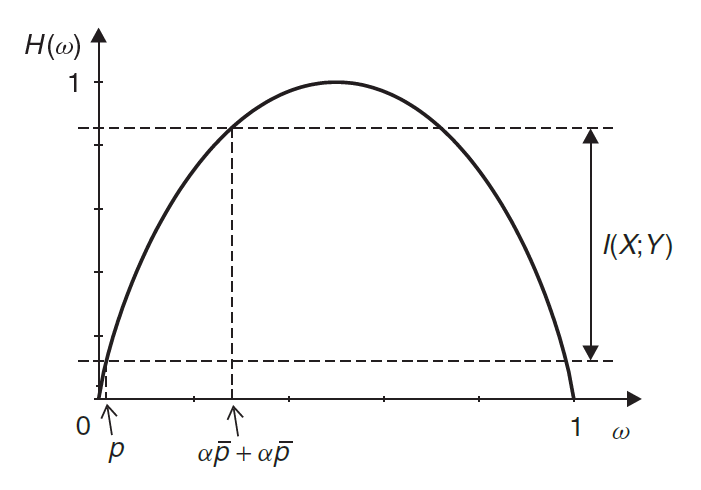
\includegraphics[width=0.6\textwidth]{./sdf/eit_87071_mutual_information_estimator/figures/mi_memoryless_binary_symmetric_channel.PNG}
	
	\caption{Graphical representation of average amount of information in the case of transmission using a binary symmetric memoryless channel. Figure from \cite{Wesolowski09}. }\label{mifigure}

\end{figure}

\subsection{Simulation Analysis}
\label{subsec:simulationmi}

\begin{figure}[H]
    \centering
        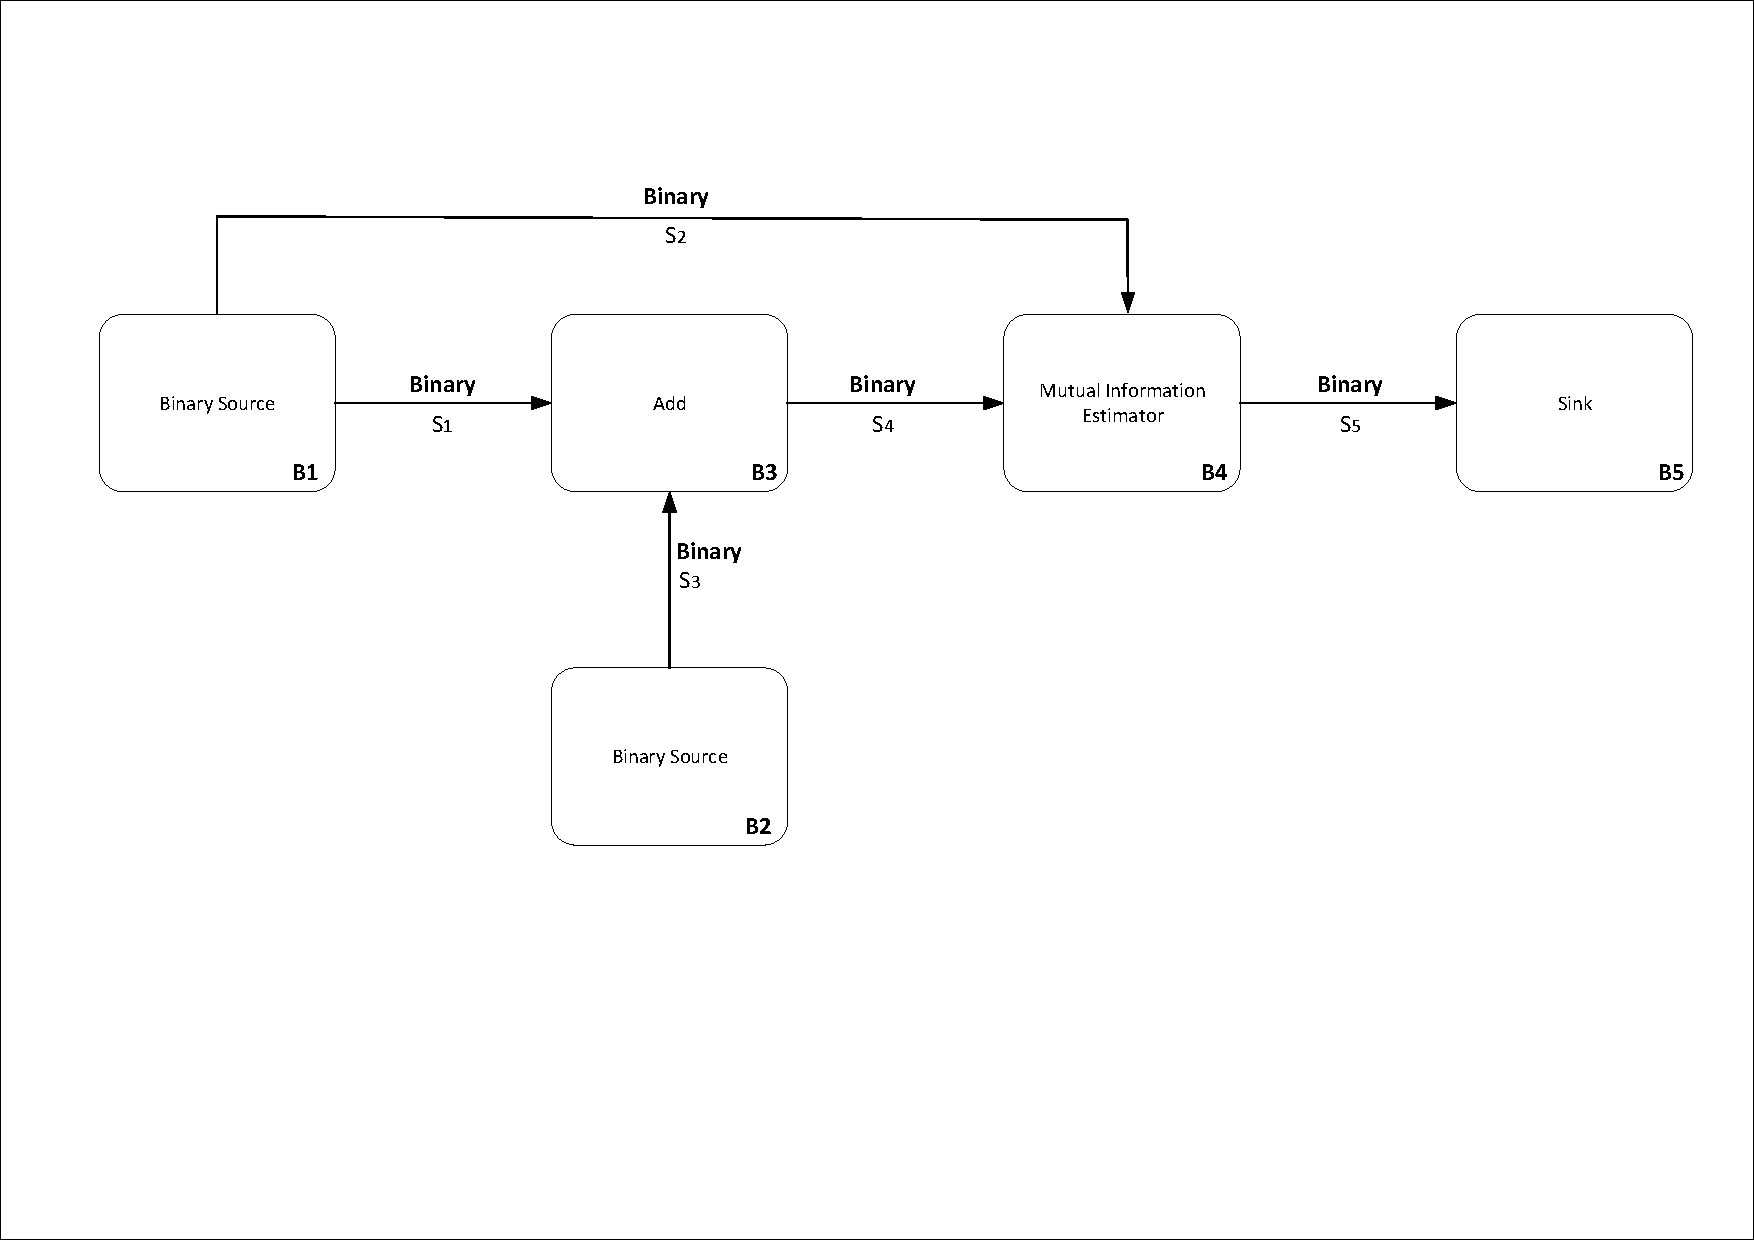
\includegraphics[clip, trim=1.0cm 6cm 1.0cm 2cm, width=0.90\textwidth]{./sdf/eit_87071_mutual_information_estimator/figures/block_diagram.pdf}
    \caption{Block diagram of the simulation implemented.}\label{fig:block_diagram}
\end{figure}

In figure \ref{fig:block_diagram} is shown the block diagram of the system implemented to test the block of mutual information estimator. In this case, the transmitter is the binary source \textbf{B1} which outputs bit 0 and bit 1 with the same probability, 0.5, randomly. The binary symmetric channel is represented by blocks \textbf{B2} and \textbf{B3}, being the first a binary source which outputs 0 with a probability $1-P_{\textrm{error}}$, where $P_{\textrm{error}}$ is defined by the user; and the second a adder block which introduces an error on the input bit sequence when the output of block \textbf{B2} is 1. Finally, \textbf{B4} is the block which estimates the mutual information between the input channel symbols and the output channel symbols and outputs a binary signal which takes value 1 when the input and output symbols are different and 0 otherwise. The functional description of this block is explained in detail in section \ref{sec_mi}.

In table \ref{tb:inputparameters2} are presented the input parameters of the system.

\begin{table}[H]
\centering
\caption{System Input Parameters}
\label{tb:inputparameters2}
\begin{tabular}{|c|c|c|}
\hline
\textbf{Parameter}                      & \textbf{Default Value}                                        \\ \hline
Perror                                  & 0.1                                                           \\ \hline
m                                       & 0                                                             \\ \hline
numberOfBits                            & 10                                                            \\ \hline

\end{tabular}
\end{table}

In table \ref{tb:signals2} are presented the system signals to implement the simulation presented in figure \ref{sim_qrng}.
\begin{table}[H]
\centering
\caption{System Signals}
\label{tb:signals2}
\begin{tabular}{|c|c|c|}
\hline
\textbf{Signal name}                            & \textbf{Signal type}                      \\ \hline
S1                                              &  Binary                                   \\ \hline
S2                                              &  Binary                                   \\ \hline
S3                                              &  Binary                                   \\ \hline
S4                                              &  Binary                                   \\ \hline
S5                                              &  Binary                                   \\ \hline
\end{tabular}
\end{table}

Table \ref{tb:signalsh} presents the header files used to implement the simulation as well as the specific parameters that should be set in each block. Finally, table \ref{tb:signalss} presents the source files.

\begin{table}[H]
\centering
\caption{Header Files}
\label{tb:signalsh}
\begin{tabular}{|c|c|c|}
\hline
\textbf{File name}                              & \textbf{Description}                                                          & \textbf{Status} \\ \hline
netxpto\_20180418.h                             &                                                                               &    \checkmark   \\ \hline
add\_20180620.h                                 &                                                                               &    \checkmark   \\ \hline
binary\_source\_20180723.h                      &                                                                               &    \checkmark   \\ \hline
mutual\_information\_estimator\_20180723.h      &                                                                               &    \checkmark   \\ \hline
sink.h                                          &                                                                               &    \checkmark   \\ \hline
\end{tabular}
\end{table}

\begin{table}[H]
\centering
\caption{Source Files}
\label{tb:signalss}
\begin{tabular}{|c|c|c|}
\hline
\textbf{File name}                                      & \textbf{Description} & \textbf{Status} \\ \hline
netxpto\_20180418.cpp                                   &                                                                               &    \checkmark   \\ \hline
add\_20180620.cpp                                       &                                                                               &    \checkmark   \\ \hline
binary\_source\_20180723.cpp                            &                                                                               &    \checkmark   \\ \hline
mutual\_information\_estimator\_20180723.cpp            &                                                                               &    \checkmark   \\ \hline
sink.cpp                                                &                                                                               &    \checkmark   \\ \hline
eit\_87071\_mutual\_information\_estimator\_sdf.cpp     &                                                                               &    \checkmark   \\ \hline
\end{tabular}
\end{table}

The system described above was implemented and it were acquired $1 \times 10^{5}$ symbols. Mutual information was calculated as well as the respective confidence intervals. The results are shown in table \ref{tb:data}.

\begin{table}[H]
\begin{tabular}{|c|c|c|c|c|c|c|}
\hline
$I(Y;X)$    & LB            & UB            & $H(Y|X)$      & $H(Y)$        & $p$           & $\bar{p}\alpha + p \bar{\alpha}$ \\ \hline
0.92226600  & 0.92392500    & 0.92060600    & 0.07772800    & 0.99999400    & 0.00954000    & 0.50147100                       \\ \hline
0.53179300  & 0.53488500    & 0.52870000    & 0.46820300    & 0.99999500    & 0.09975000    & 0.49871100                       \\ \hline
0.27601000  & 0.27878100    & 0.27324000    & 0.72398300    & 0.99999400    & 0.20103000    & 0.50147700                       \\ \hline
0.11982400  & 0.12183600    & 0.11781100    & 0.88017600    & 0.99999900    & 0.29909000    & 0.50052600                       \\ \hline
0.02746750  & 0.02848050    & 0.02645450    & 0.97253100    & 0.99999800    & 0.40274000    & 0.50074900                       \\ \hline
2.34E-08    & 9.71E-07      & -9.24E-07	    & 1.00000000    & 1.00000000    & 0.49991000    & 0.50000000	                   \\ \hline
0.0285718   & 0.0296043     & 0.0275392     & 0.9714280     & 1.0000000     & 0.5991800     & 0.4999960                        \\ \hline
0.1187460   & 0.1207510     & 0.1167410     & 0.8812540     & 1.0000000     & 0.7000300     & 0.5001840                        \\ \hline
0.2729990   & 0.2757600     & 0.2702380     & 0.7269990     & 0.9999980     & 0.7974500     & 0.5008510                        \\ \hline
0.5310040   & 0.5340970     & 0.5279110     & 0.4689960     & 1.0000000     & 0.9000000     & 0.4996960                        \\ \hline
0.9182140   & 0.9199120     & 0.9165160     & 0.0817859     & 1.0000000     & 0.9898500     & 0.5001960                        \\ \hline
\end{tabular}
\caption{Results acquired for $1 \times 10^{5}$ symbols acquisition.}
\label{tb:data}
\end{table}

After that the second line data from table \ref{tb:data} was chosen to represent graphically as shown in figure \ref{fig:datafig}.

\begin{figure}[h]
    \centering
        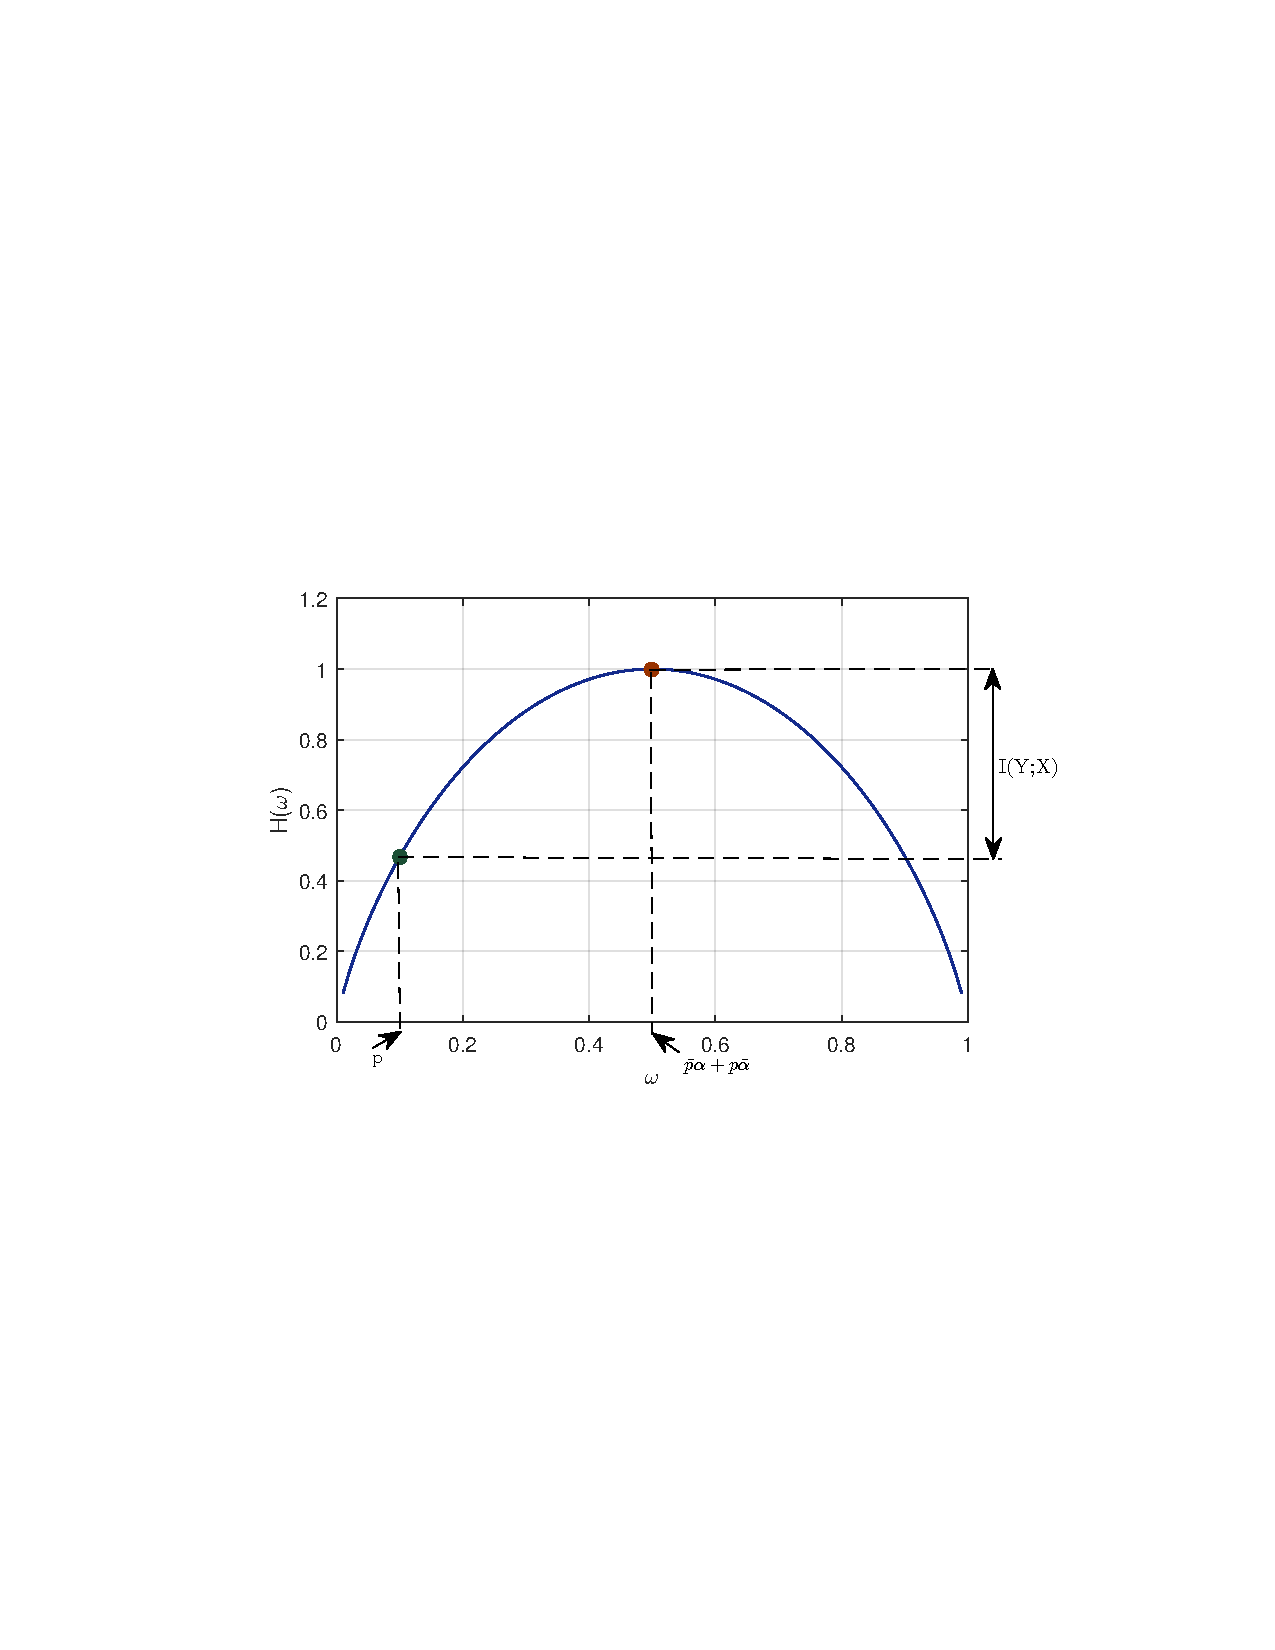
\includegraphics[clip, trim=1.0cm 9cm 1.0cm 9cm, width=0.90\textwidth]{./sdf/eit_87071_mutual_information_estimator/figures/fig1.pdf}
    \caption{Numerical results representation for mutual information calculation. $I(Y;X) = H(Y) - H(Y|X) = 0.5318$; $H(Y|X) = 0.4680$; $H(Y) = 1.0000$; $p=0.0998$; $\bar{p}\alpha + p \bar{\alpha} = 0.4987$.}\label{fig:datafig}
\end{figure}

Results shown in figure \ref{fig:datafig} meet the theoretical representation shown in figure \ref{mifigure}. Moreover, mutual information was calculated for a binary symmetric channel using different channel error probabilities ($p$), theoretically, using equation \ref{eq:mi_bsc}. Both, theoretical and numerical values with the respective confidence intervals of mutual information were plotted in figure \ref{fig:theornum}. As one can see in the figure, the numerical results meet the theoretical values of mutual information, which means that the mutual information estimator has the expected performance.

\begin{figure}[h]
    \centering
        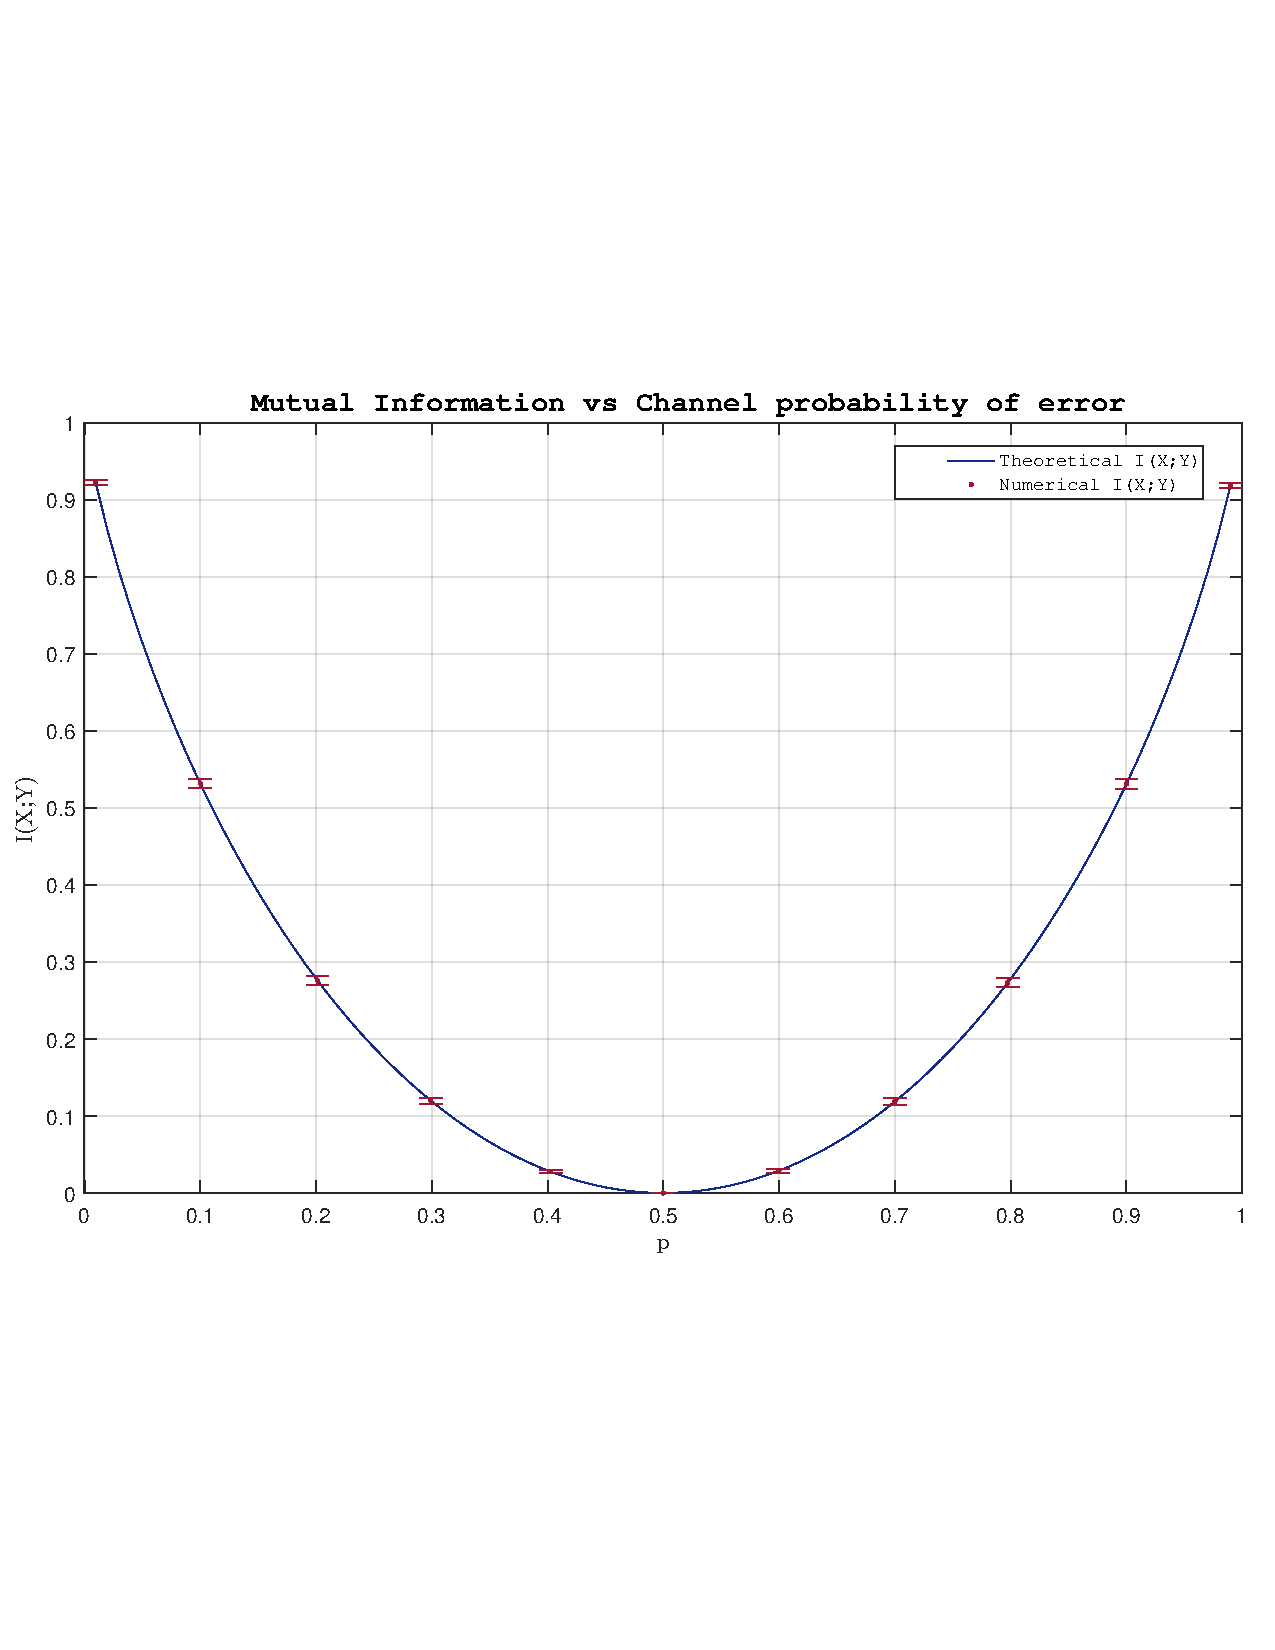
\includegraphics[clip, trim=0.05cm 6cm 0.5cm 6cm, width=0.90\textwidth]{./sdf/eit_87071_mutual_information_estimator/figures/fig2.pdf}
    \caption{Numerical values of mutual information for different channel probability errors Vs theoretical mutual information.}\label{fig:theornum}
\end{figure}




% bibliographic references for the section ----------------------------
\clearpage
\printbibliography[heading=subbibliography]
\end{refsection}
\addcontentsline{toc}{subsection}{Bibliography}
\cleardoublepage
% --------------------------------------------------------------------- 